%% You must start off the LaTeX document with \documentclass{<document type>}
\documentclass{article} % try twocolumn and change font

%% Template for importing package
% \usepackage[options]{package}

%% Similar to importing packages/libraries for programming languages
\usepackage[utf8]{inputenc} % important so you can compile you document
\usepackage{hyperref} % stylize links
\usepackage{graphicx} % import graphics
\usepackage{setspace} % allow double spacing
\usepackage{amsmath} % allow math equations
\usepackage[a4paper]{geometry} % change paper
\usepackage{booktabs} % nicer tables

%% Uncomment the below two packages to get Times New Roman
% \usepackage[T1]{fontenc}
% \usepackage{mathptmx}

%% Try some fonts below by uncommenting them individually
% \renewcommand*{\familydefault}{\sfdefault}
% \renewcommand*{\familydefault}{\ttdefault}
% \renewcommand*{\familydefault}{\rmdefault}
% \renewcommand*\rmdefault{iwona}

% These three commands define your title but do not actually display it
\title{BioDSP \LaTeX~Demonstration}
\author{Eric Leung}
\date{July 16th, 2015}

%% Uncomment the command below to add double spacing to the document
% \doublespacing

\begin{document} % This command is similar to the <body> tag to HTML

% The basic syntax of a command:
% \commandname[option1,option2,...]{argument1}{argument2}...

\maketitle % Used to actually display the title items defined above.

\phantomsection{} % anchor manual positioning
\tableofcontents % make table of contents

\section{Outline}

Here is an outline to how to use \LaTeX. The things I will cover are:

\begin{itemize}
    \item setting up a \LaTeX~document
    \item sections
    \item comments % And like magic, you can't see this!
    \item text formatting
    \item equations
    \item lists and descriptions
    \item tables
    \item importing graphics
    \item footnotes
    \item bibliographies and BibTeX
\end{itemize}

{\LARGE If you were to get one thing out of this entire document, I'd say it
should be the Wikipedia Wikibooks for
\LaTeX{}\footnote{\url{https://en.wikibooks.org/wiki/LaTeX}}; it is an amazing
resource!}

\subsection{Beginnings}

The absolute minimal \LaTeX{} code you need to make a document is the following:
% This environment tells LaTeX to display literally what is there
\begin{verbatim}
\documentclass{article}

\begin{document}
Hello World. Space    does matter here.
\end{document}
\end{verbatim}

But there is much more to a document than ``Hello World.'' I will not get into
the technical details of how a \verb+.tex+ file gets converted into a PDF but
you can find out more here: \url{https://en.wikibooks.org/wiki/LaTeX/Basics}.

An analogy for what \LaTeX{} is as a markup language is comparing it to HTML\@.
HTML defines the structure of the webpage where the browser displays the content
while one form to display \LaTeX{} is a PDF\@.

% An example of how LaTeX handles spaces
It does not matter whether you
enter one or several             spaces
after a word.

An empty line starts a new
paragraph.

\paragraph{Text Formmating} You can put \emph{emphasis} on words. You can
\textbf{bold} them as well. Another way to grab people's attention is to write
{\LARGE large font here}. Or you can be really subtle and make your text really
{\tiny small}.

\paragraph{Special Characters} The following characters need a backslash (i.e.{}
``\textbackslash'') in order to render correctly: \# \$ \% \^{} \& \_ \{ \} \~{}
\textbackslash{}.

\subsubsection{Why Use \LaTeX}

I borrowed these arguments verbatim from Dr.\ Kent H.\ Lundberg at
MIT~\cite{Lundberg:aa}.

\begin{itemize}
    \item \TeX{} math mode is a thing of beauty. Equations come out looking
        correct.  Mathematical expressions in Word are treated as an
        afterthought. Equation editor is \textbf{evil}.
    \item \TeX{} is guaranteed to be bug free. The author, Stanford Professor
        Donald Knuth, will send you a reward check\footnote{Here's what one of
        those reward checks look like
        \url{http://truetex.com/knuthchk.htm}}\footnote{And the Wikipedia article on
        it \url{https://en.wikipedia.org/wiki/Knuth_reward_check}} if you find a
        bug.  The reward is currently \$327.68 (that is, $2^{15}$ cents).
    \item \TeX{} is free (as in beer) and free (as in speech).
    \item \TeX{} has real comments. Anyone who doesn't comment their code is an
        ass.
    \item \TeX{} provides a full, turing-complete, language. The text produced
        by your input file can be the result of conditionals (which I use to
        reuse sections in different documents) or the result of complicated
        calculations. In the TeXbook, Knuth demonstrates the power of the \TeX{}
        language by defining the \verb+\primes{n}+ command, which calculates and
        prints the first n primes (see page 218).
    \item There are no \TeX{} ``macro'' viruses. You can safely receive \TeX{}
        documents by email and not worry about it reading your Outlook address
        book and mailing copies of itself to all your friends.
    \item \TeX{} has no GUID (Globally Unique Identifier). Word documents are
        embedded with a code that can be traced back to your computer (the
        police captured the author of the Melissa virus by tracing his GUID).
        Big brother Bill is watching!
    \item \TeX{} versions are not incompatible. The file format has never
        changed. I have TeX files from 1989 that work without problem in the
        latest version of \TeX{}.
    \item There is no undo feature in \TeX{}. This is a good thing. No one can
        ever seen earlier versions of your TeX document by pressing the Undo
        button.
    \item \TeX{} documents are small and lean. What's the smallest Word file on
        your computer?
\end{itemize}

If those were not enough, here is a graphic in Figure~\ref{fig:MS_Word} that
will hopefully convince you \LaTeX~is the way to go.

\begin{figure}[ht]
\centering
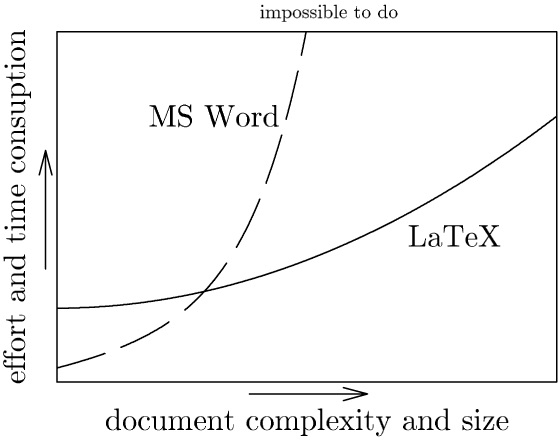
\includegraphics[width=\columnwidth]{./images/miktex.jpg}
\caption{``Although Word is a useful and practical tool for writing short and
(very) simple documents, it becomes too complex or even unusable when one wants
the word processor to do more complicated tasks. Moreover, many rather commonly
needed features, like user-customised automated numbering or various automated
indexes, cannot be created using Word at all. \LaTeX{} does require more effort
and time to learn to use even for simpler tasks, but once learned, difficult
tasks can be accomplished rather easily and straightforwardly.''
\cite{Pinteric:2004aa}}
\label{fig:MS_Word}
\end{figure}

\section{Tables!}

You can find an example of a table below in Table~\ref{tableExample}. I have to
admit I used this website to help me make this table:
\url{http://truben.no/table/}.

\begin{table}[ht]
\centering
    \begin{tabular}{lll}
    Name     & University                      & State \\ \toprule
    Cuthbert & Portland State University       & OR    \\
    Hermine  & Ohio State University           & OH    \\
    Luann    & University of California, Davis & CA    \\
    \end{tabular}
    \caption{A simple example of a table~\label{tableExample}}
\end{table}

\section{Typesetting Math}

\LaTeX{} is very powerful when it comes to typesetting mathematical equations
compared to Microsoft Word. Here are 17 equations which supposedly changed the
world~\cite{Nisen:2012aa}.
\begin{align}
& \text{The Pythagorean Theorem}
& a^2 + b^2 = c^2 \\
%
& \text{Logarithm and Its Identities}
& \log(xy) = \log(x) + \log(y) \\
%
& \text{Fund. Theorem of Calculus}
& \frac{df}{dt} = \lim_{h \to 0} \frac{f(t+h) - f(t)}{h} \\
%
& \text{Newton's Law of Gravitation}
& F = G \frac{m_1 m_2}{d^2} \\
%
& \text{Origin of Complex Numbers}
& i^2 = -1 \\
%
& \text{Euler's Form.\ for Polyhedra}
& F - E + V = 2 \\
%
& \text{The Normal Distribution}
& \phi(x) = \frac{1}{\sqrt{2\pi\sigma}}e^{\frac{(x-\mu)^2}{2\sigma^2}} \\
%
& \text{The Wave Equation}
& \frac{\partial^2 u}{\partial t^2} = c^2 \frac{\partial^2 u}{\partial x^2} \\
%
& \text{The Fourier Transform}
& \hat f(\xi) = \int_{-\infty}^\infty f(x) e^{-2 \pi ix \xi}\, dx \\
%
& \text{Navier-Stokes Equation}
& \rho \left(\frac{\partial \nu}{\partial t} + \nu \cdot \nabla \nu \right) = -\nabla p + \nabla \cdot T + f \\
%
& \text{Maxwell's Equations}
& \nabla \cdot \mathbf{E} = 0, \nabla \time \mathbf{E} = -\frac{\partial \mathbf{B}}{\partial t} \\
%
& 
& \nabla \cdot \mathbf{B} = 0, \nabla \time \mathbf{B} = -\frac{1}{c^2}\frac{\partial \mathbf{E}}{\partial t} \nonumber \\
%
& \text{2\textsuperscript{nd} Law of Thermodynamics}
& dS \ge 0 \\
%
& \text{Einstein's Theory of Relativity}
& E = mc^2 \\
%
& \text{The Schrodinger Equation}
& i \hbar \frac{\partial}{\partial t} - \Psi = \hat H \Psi \\
%
& \text{Shannon's Infor. Theory}
& H = -\sum p(x) \log p(x) \\
%
& \text{Logistic Mod.\ for Pop. Growth}
& x_{t+1} = kx_t (1 - x_t) \\
%
& \text{Black-Scholes Model}
& \frac{1}{2} \sigma^2 S^2 \frac{\partial^2 V}{\partial S^2} + rS \frac{\partial V}{\partial S} + \frac{\partial V}{\partial t} - rV = 0
\end{align}

A matrix in text must be set smaller:
$\bigl(\begin{smallmatrix}
a&b \\ c&d
\end{smallmatrix} \bigr)$
to not increase leading in a portion of text.

A great place to find out more on how to typeset math can be found here:
\url{https://en.wikibooks.org/wiki/LaTeX/Mathematics}.

\section{How to Deal with Bibliographies}

Here's a web page with all sorts of reference styles:
\url{http://www.cs.stir.ac.uk/~kjt/software/latex/showbst.html}.

\section{Resources}

Here's a list of websites I found to be useful.

\begin{itemize}
\item \url{http://schneider.ncifcrf.gov/latex.html}
\item \url{http://mirror.utexas.edu/ctan/info/lshort/english/lshort.pdf}
\end{itemize}

\bibliographystyle{is-unsrt}
\bibliography{ref}

\end{document}
